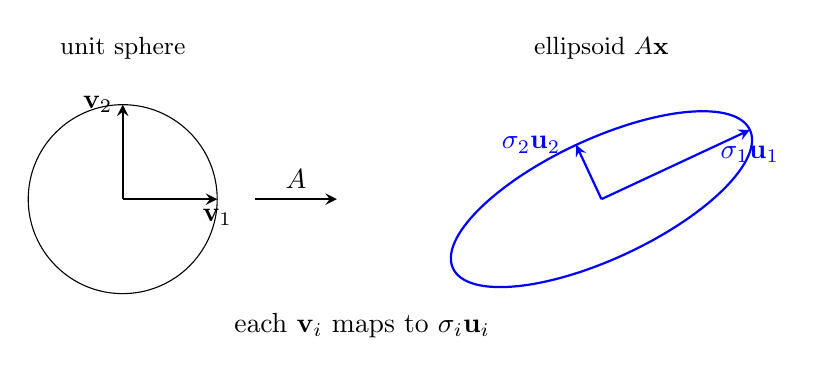
\begin{tikzpicture}[scale=0.8,>=stealth]
\node at (0,2.4) {\small unit sphere};
\draw (0,0) circle (1.5);
\draw[->,thick] (0,0)--(1.5,0) node[below]{$\mathbf v_1$};
\draw[->,thick] (0,0)--(0,1.5) node[left]{$\mathbf v_2$};
\draw[->,thick] (2.1,0)--(3.4,0) node[midway,above]{$A$};
\begin{scope}[xshift=7.6cm]
\node at (0,2.4) {\small ellipsoid $A\mathbf x$};
\draw[blue,thick,rotate=25] (0,0) ellipse (2.6 and 0.95);
\begin{scope}[rotate=25]
\draw[->,thick,blue] (0,0)--(2.6,0) node[below=2pt]{$\sigma_1\mathbf u_1$};
\draw[->,thick,blue] (0,0)--(0,0.95) node[left=2pt]{$\sigma_2\mathbf u_2$};
\end{scope}
\end{scope}
\node at (3.8,-2.0) {each $\mathbf v_i$ maps to $\sigma_i\mathbf u_i$};
\end{tikzpicture}
